\documentclass{scrartcl}

\usepackage[T1]{fontenc}
\usepackage[utf8]{inputenc}

\title{Mobile Dev A3.2P}
\author{Daniel Coady (102084174)}
\date{20/09/2019}

\usepackage{graphicx}

\begin{document}

\maketitle

\section*{Part 1}

\begin{figure}[h]
    \centering
    
\includegraphics[scale=0.7]{images/screen1.png}
    \caption{Screenshot of the application working}
\end{figure}
\begin{figure}[h]
    \centering
    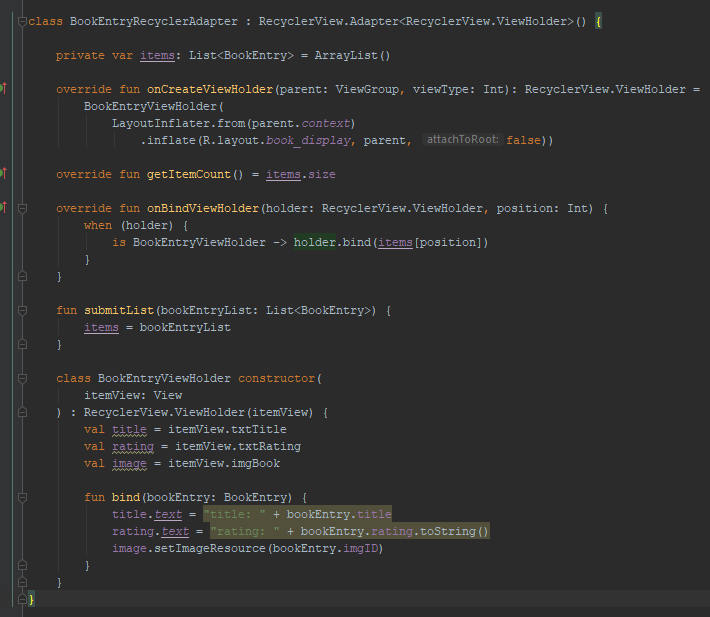
\includegraphics[scale=0.7]{images/screen2.png}
    \caption{Screenshot of the adapter code}
\end{figure}

\pagebreak

\section*{Part 2}

\subsection*{Fragments vs Activities}
Fragments are groups of views within an activity which can be reused in other places within
the application. There can be multiple fragments in an activity that form the larger UI
and each of these fragments have their own lifetime. The key difference between the two
is that while activities can contain fragments, fragments cannot contain activities. As
well as this, it is important to note that unlike activities which are slow to load,
fragments are far faster to load which makes switching out small parts of the UI much
better and faster than if done with just activities.

\subsection*{What is a FragmentManager and a fragment transaction}
Fragment transactions are how we are able to add, replace, or remove fragments from an
activity. The FragmentManager then allows us to handle these transactions.

\subsection*{How are intents used to transition between activities?}
Intents are our way of stating what activity we wish to launch and what data we wish to
send along with it. The way we do this is by constructing the intent by passing through
the class that we wish to instantiate and then adding any of the extra data we wish
to send to the new activity.

\end{document}
